% !TeX root = RJwrapper.tex
\title{Comparison of Spatial Interpolation Methods for Air Pollution
Prediction\texttt{:} gstat and mgcv}
\author{by Hyesop Shin}

\maketitle

\abstract{%
Understanding the association between pollution exposure and the
deleterious effect on population health is a vital precursor for
modelling. However, there has been less comparisons of spatial
interpolations for pollution predictions due to different assumptions
and mathematical processes. In addition, SI has been provided in a
coarse temporal scale which is difficult to understand the dynamics of
exposure by mobility patterns and seasonal effects. This paper aims to
compare spatial interpolation methods to predict air pollution at a
finer temporal scale. 57 pollution stations around Seoul, S.Korea were
collected for the comparison between Universal Kriging and Generalised
Additive Model, with additional weights on road layers as an effect of
roadside pollution fields. Neither of the interpolation methods was
noticeably superior to the other, but the sparse station data meant that
only very smoothed large-scale fields could be recovered, which did not
accurately represent the extremes observed at individual stations..
}

\hypertarget{introduction}{%
\subsection{Introduction}\label{introduction}}

Population health has been seriously threatened by daily ambient air
pollution in South Korea. Despite the efforts to legislate national
pollution standards, daily peaks in recent winters and springs have
already exceeded the standards countless times. During 5th-8th March
2019, the entire country experienced over 200µg/m\textsuperscript{3} of
PM\textsubscript{10} and smog episodes; the national authorities warned
everyone to reduce outdoor activities. As most of Seoul's areas tend to
experience disastrous levels of pollution frequently, residents can be
exposed to air pollution unconsciously, which in the long-term can lead
to respiratory or cardiovascular ailments \citep{Zhang2013}. Thus,
understanding the spatial and temporal aspects of air pollution and its
relationship with exposure is crucial.

Exposure research has exploited spatial interpolation (SI) to
investigate the relationship between ambient air pollution and
population exposure in a spatial context -- ``which places have high air
pollution?'' and ``how many people can potentially become unwell from
high episodes?''. SI is a statistical method that can compute pollution
fields over a wide area with a given set of point measurements. SI can
mainly be split into a group that follows the assumption of spatial
autocorrelation (e.g.~Inverse Distance Weighted (IDW), Kriging), and a
group on statistical inference e.g.~generalised linear models and
generalised additive models \citep{Wood2019}. Methods that take spatial
autocorrelation into account assume that the values tend to be more
similar when closer together, whereas methods that use (spatial)
statistical inference delineate the inferential surfaces over a region
by minimising the residuals of the model.

However, when air pollution monitoring stations such as those in Seoul
are small in number compared to the size of the city, the estimation of
the potential population at risk due to air pollution can be completely
different depending on the measurement method used \citep{Wu2019}.
\citet{Wong2004} used four spatial interpolation methods -- spatial
averaging, nearest neighbour, IDW, and Kriging - to estimate children's
exposure to air pollution across the USA. The outcomes of the four
methods only showed a small difference of PM\textsubscript{10} and
O\textsubscript{3} where the monitoring stations were denser, for
example in the northeastern cities and urban California, but was
difficult to predict in the mountainous regions and high-altitude zones.
\citet{Aalto2013} compared a Generalised Additive Model (GAM) and an
Ordinary Kriging (OK) to predict monthly mean temperature and
precipitation and found that the GAM outperformed other methods by a
small amount but the biased distribution of stations (``concentrated in
the urban areas'' of Finland) might have evened out the RMSE measures.

In addition, previous studies have provided tentative estimates of
population risk based on annual or monthly statistics, but the
aggregated figure lacks the potential for including acute injuries after
an abrupt pollution rise, which may be more severe. However, there is
likely to be a greater difference when the population at risk is
measured at a finer temporal scale. This might support guidelines for
surveillance of short-term exposure.

This chapter aims to compare spatial interpolation methods that can
support estimating population exposure to daily air pollution in Seoul.
This study compared Universal kriging (UK), Generalised additive model
(GAM), UK with additional road effect, and GAM with additional road
effect to model PM\textsubscript{10}, and NO\textsubscript{2} in Seoul
as an intermediate phase of pollution modelling. Compared to previous
studies, this chapter generates outcomes on a 12-hour basis to
understand the daily cycle of the pollution over the city and
superimposes road effects to take into account small scale variables
that might be neglected in the typical spatial interpolation outcomes.

\hypertarget{data}{%
\subsection{Data}\label{data}}

This article explores the spatial and temporal patterns of pollution in
Seoul as well as the extent to which background and roadside stations
are similar or different. The NIER (National Institute of Environmental
Research) provided 6 pollutants, PM\textsubscript{10},
PM\textsubscript{2.5}, NO\textsubscript{2}, CO, SO\textsubscript{2},
O\textsubscript{3}, which were released as an hourly aggregation. This
study selected PM\textsubscript{10} as the main source that can causally
result in human cancer and NO\textsubscript{2} as the main source that
harms respiratory symptoms, whether constantly or instantaneously
\citep{WHO2013}.

Pollution data were collected from two different types of stations:
background stations (installed on the rooftops of district offices), and
roadside stations (close to the major roads which are strongly affected
by nearby traffic). This study took into account 57 urban background
stations and 19 roadside stations that were within 10km from the city
boundary (see Figure \ref{fig:pollution_stations}). Amongst these 76
stations, Seoul itself had 25 background stations and 15 roadside
stations. Roadside data were retrieved from the 19 stations installed on
the roads near the city centre, 8-lane junctions, and a highway
entrance. The possible download period was between 01/01/2010 01:00 and
01/01/2018 00:00. Units are measured in ppb (parts per billion) for
NO\textsubscript{2}, and µg/m\textsuperscript{3} for
PM\textsubscript{10}.

\begin{figure}[htbp] 
\begin{center} 
    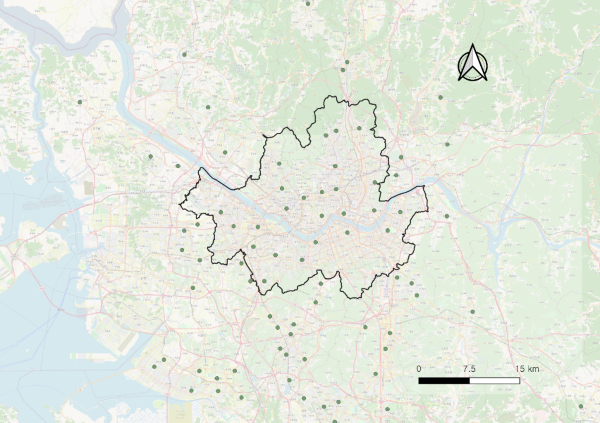
\includegraphics[width=.7\textwidth]{Figures/pollution_stations.png}
\end{center}
 \caption{57 Background pollution stations that are considered for spatial interpolation (boundary area: Seoul)} 
 \label{fig:pollution_stations} 
\end{figure}

\hypertarget{kriging-conceptual-framework}{%
\subsection{Kriging: Conceptual
Framework}\label{kriging-conceptual-framework}}

Kriging is a geostatistical method that interpolates an unknown location
using the characterized mean and variance structures
\citep{Kumar2007, Kim2014}. It assumes that the overall mean, distance,
and variance of all observations are spatially autocorrelated from
Tobler's First Law of Geography: ``Everything is related to everything
else, but nearer things are more related than distant things''. For
example, pollution concentrations less than 1 metre apart are likely to
be similar, but less likely when the distance becomes larger. This
context of the variability between the two values and their grouped
distances (e.g.~0-100m, 101-200m) can be structurally applied over the
region with a conceptual semivariogram. Once the semivariogram is
produced, then the kriged map is produced together with an error map.

To create a kriged map, there are a few steps to follow: 1) modelling an
empirical semivariogram, 2) fitting the empirical model with a
mathematical model, and 3) choosing the type of kriging according to the
fit of the assumptions (i.e.~data normality, stationarity, and whether
the data has trends).

\hypertarget{understanding-semivariograms}{%
\subsubsection{Understanding
Semivariograms}\label{understanding-semivariograms}}

Spatial autocorrelation (or spatial dependency) is assessed by a
semivariogram. Semivariograms apply the squared differences of
measurements against distances between pairs of data points (see
Equation\textasciitilde{}\ref{eq:semivariogram}). This means that all
the pollution values at the 57 stations are compared between one
another, and once calculated, the semivariogram is drawn. The conceptual
semivariance can be estimated as below.

\begin{equation}
\label{eq:semivariogram}
\gamma(h)= \frac{1}{2N}(h) \sum_{i=1}^{N(h)}{Z(s_i) - Z(s\textsubscript{i} + h)\textsuperscript{2}}
\end{equation}

\begin{itemize}
 \setlength\itemsep{0em}
    \item N(h)= number of pairs of observation points with distance \texttt{h}
    \item Z = field that holds a height or magnitude value for each point (z-values)
    \item Z(s\textsubscript{i})and Z(Si+h) = sample data pairs at a distance \texttt{h} \citep{Luo2008}
\end{itemize}

Directions are not considered in the current formula; however, this can
be taken into account depending on the aspect of the study, for example,
if the wind direction is dominantly affecting the pollution
concentrations.

\begin{figure}[hbt!]
\begin{center} 
  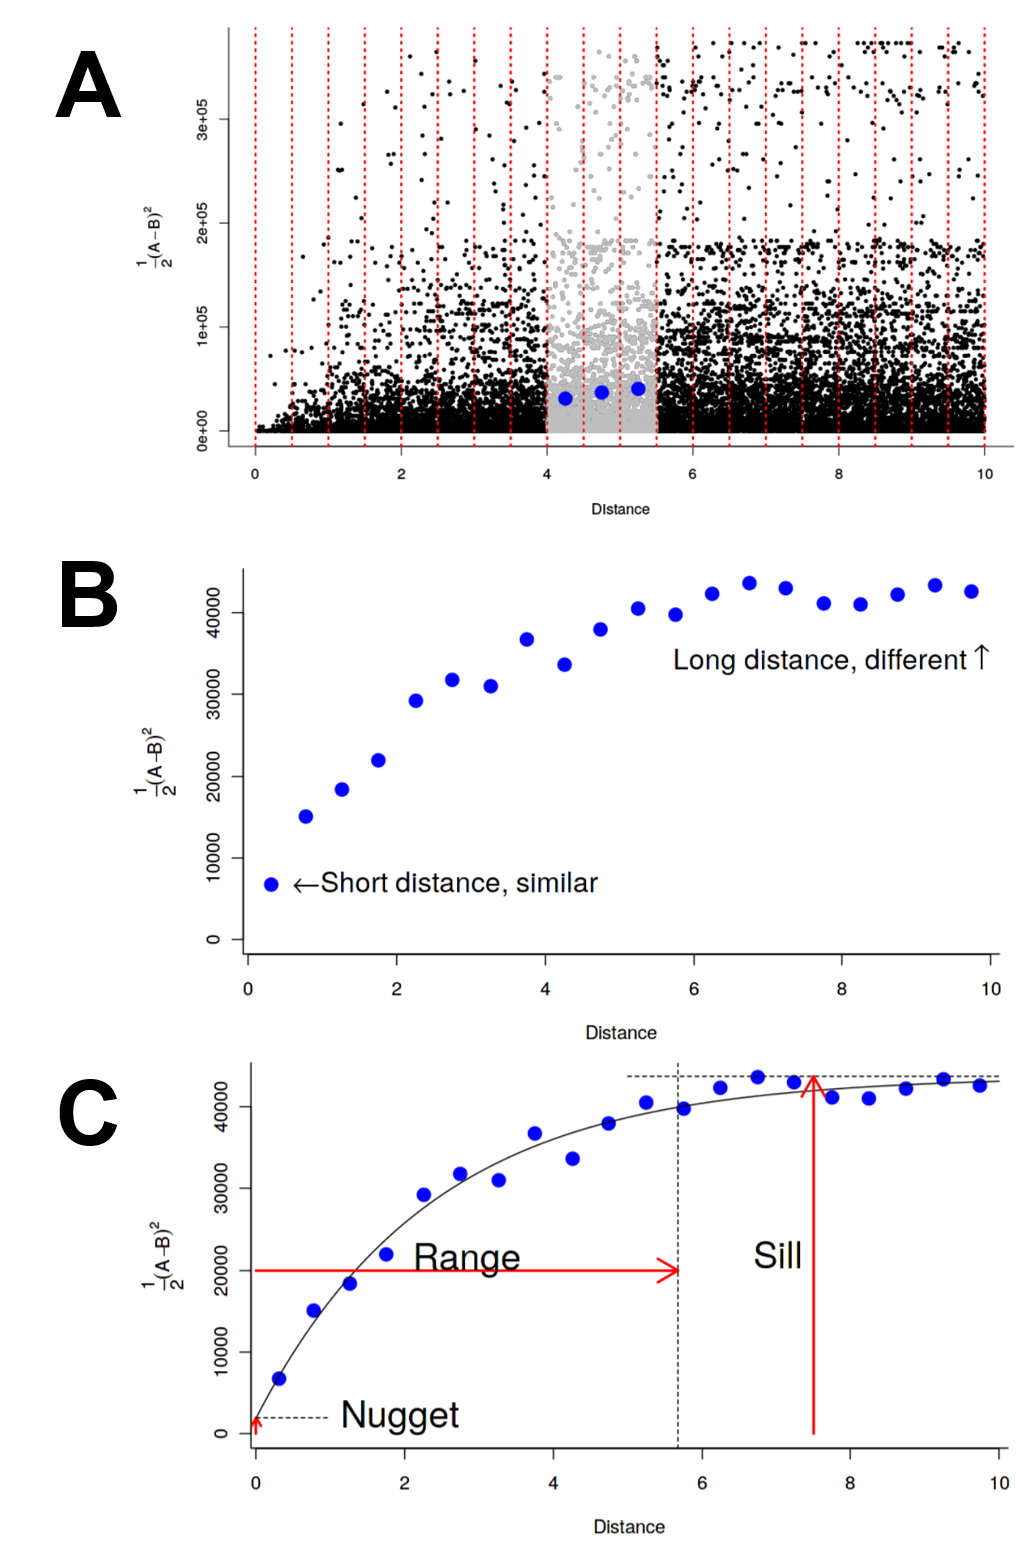
\includegraphics[width=.5\textwidth]{Figures/semivariogram.png}
\end{center} 
\caption[Conceptual process of kriging measurements]{Conceptual process of kriging measurements $($captured from Datacamp.com lectures$)$} 
\label{fig:semivariogram} 
\end{figure}

Figure \ref{fig:semivariogram} explains the process to generate a
semivariogram. First, the distance against half-squared distances
between all pair points is plotted in the variogram cloud (see Figure
\ref{fig:semivariogram}a). The dots in the variogram cloud are allocated
to an arbitrary number of imaginary bins (10 bins are used for this
study). The mean of each bin becomes a representative point which
normally has an upward trend as the distance increases to some extent
and then levels off (see Figure \ref{fig:semivariogram}b). This means
that the closer the distance, the more similar the values are, and vice
versa. Finally, an asymptotic curve, termed semivariogram, is drawn
through the points (see
Figure\textasciitilde{}\ref{fig:semivariogram}c).
Range\footnote{The distance at which a spatial correlation exists.},
partial
sill\footnote{The upper limit of the semivariogram is the sill. A Sill minus a nugget is termed a partial-sill},
and
nugget\footnote{Represents short scale randomness or noise in the regionalised variable [@Camana2020]}
are the key parameters inside the model, and the kriged map is drawn
based on the semivariogram \citep{Law2019}.

\begin{verbatim}
  myVario[[length(myVario)+1]] <- variogram(top.jan[[i]] ~ 1, top.jan, cutoff = 30000, width = 3000)
  myList[[i]]  <- fit.variogram(myVario[[i]], 
                                vgm(psill = 100,
                                    nugget= 15,
                                    model = "Ste"),
                                fit.kappa = TRUE, fit.method = 6)
\end{verbatim}

\bibliography{RJreferences.bib}

\address{%
Hyesop Shin\\
MRC/CSO Social and Public Health Sciences Unit, University of Glasgow\\%
Berkeley Square, 99 Berkeley Street, Glasgow, G3 7HR\\
%
\url{https://www.gla.ac.uk/researchinstitutes/healthwellbeing/staff/hyesopshin/}\\%
%
\href{mailto:hyesop.shin@glasgow.ac.uk}{\nolinkurl{hyesop.shin@glasgow.ac.uk}}%
}
